\documentclass[12pt, a4paper, twoside]{article}

%% Preamble
\usepackage{pdfpages}           % Para incluir PDFs
\usepackage{graphicx}           % Para gráficos
\usepackage{subfiles}           % Para manejar subarchivos
\usepackage{hyperref}           % Para enlaces
\usepackage{listings}           % Para código fuente (ajusta lenguaje)
\usepackage{verbatim}
\usepackage[backend=bibtex,style=numeric]{biblatex} % Para citas numéricas
\addbibresource{references.bib} % Cargar archivo .bib
\usepackage{url}
\usepackage{float}


\usepackage{geometry}           % Para ajustar márgenes

% Ajustes de márgenes
\geometry{
	left=3cm,       % Margen izquierdo
	right=3cm,      % Margen derecho
	top=2.5cm,      % Margen superior
	bottom=2.5cm,   % Margen inferior
	headheight=15pt, % Altura del encabezado
	twoside          % Para documentos a dos caras
}


\graphicspath{{images/}{../images/}} % Ruta para imágenes

\begin{document}
	
	%% Cover
	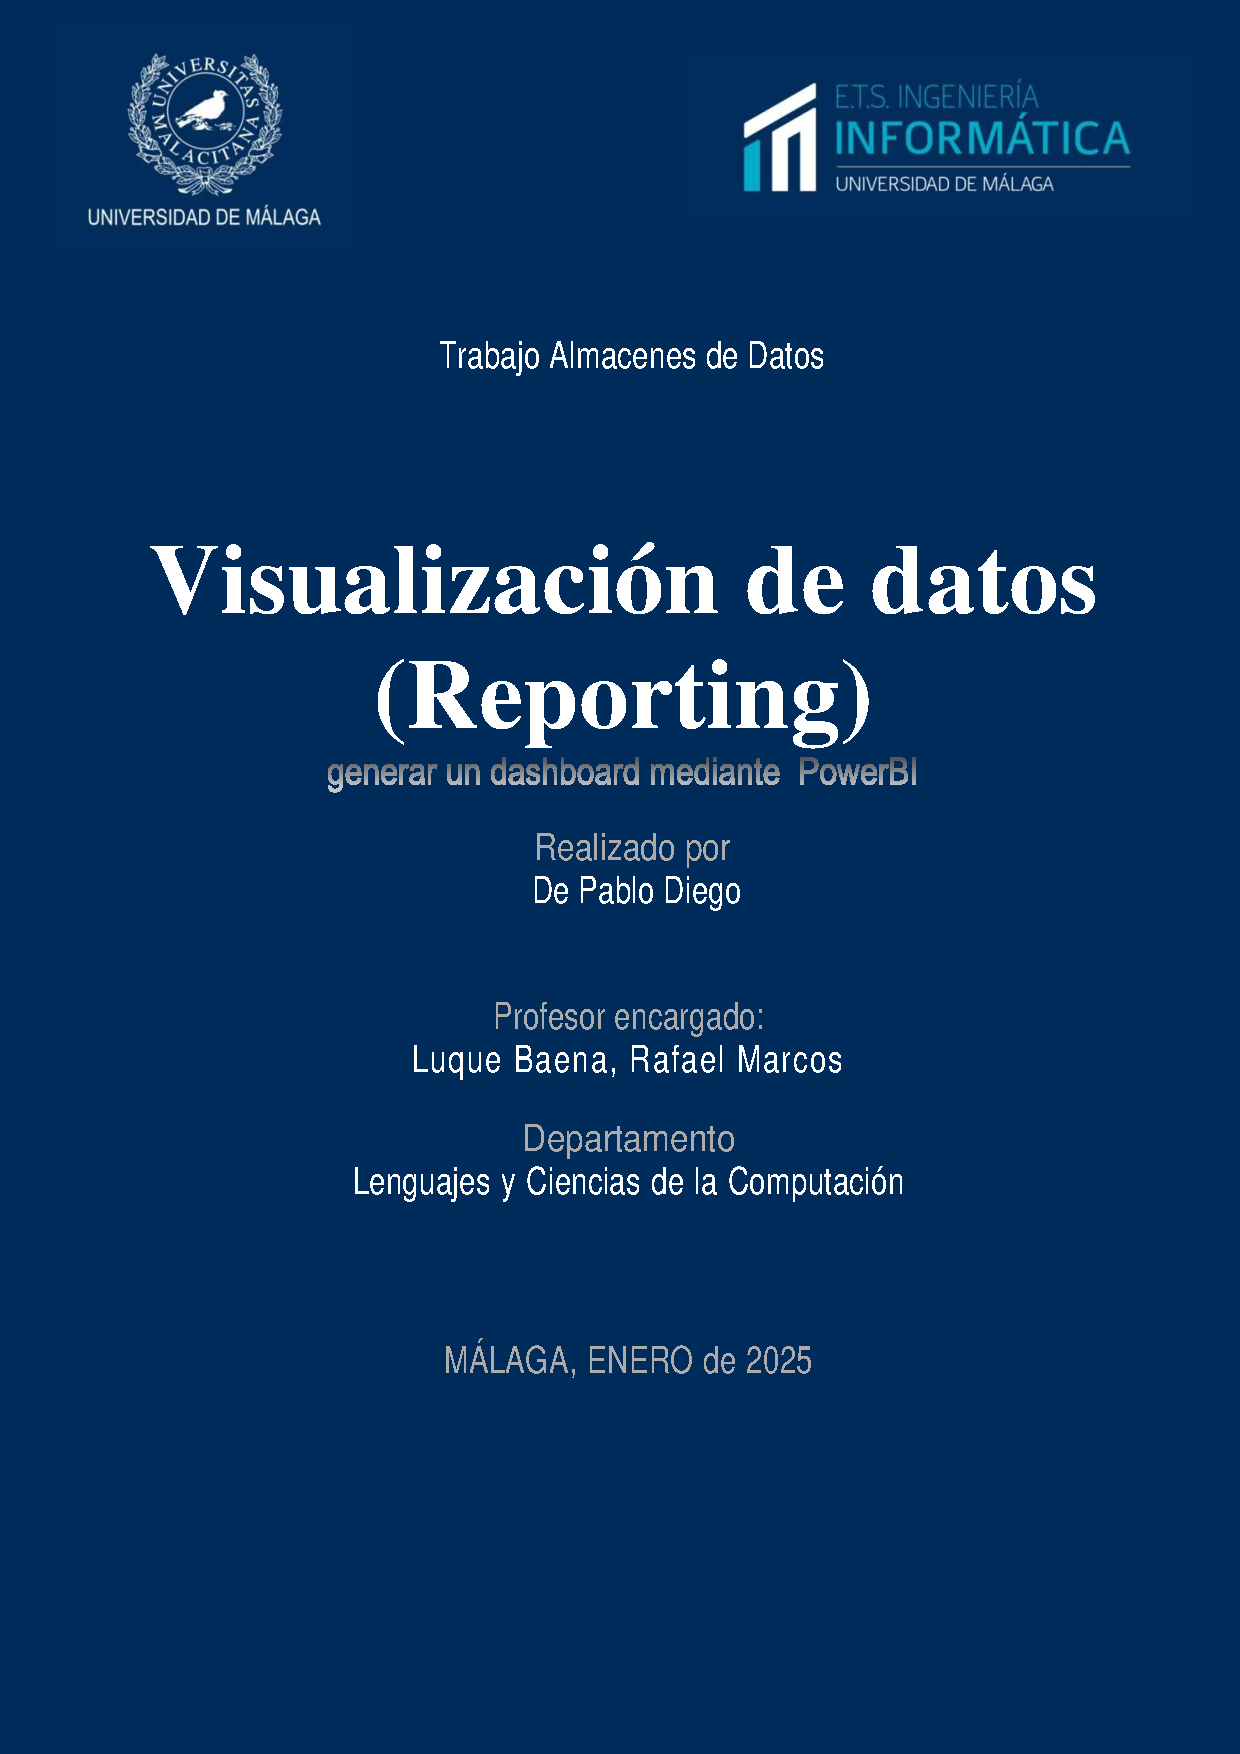
\includepdf[noautoscale=true, width=\paperwidth]{cover.pdf}
	
	%% Title
	\clearpage
	\setcounter{page}{1}
	
\includepdf[noautoscale=true, width=\paperwidth]{title.pdf}
	
	%%%%%%%%%%%%%%%%%%%%%%%%%%%%%%%%%%%%%%%%%%%%%%%%%%%%%%%%%%%%%%%%%%%%%%%%%%%
	
	% Índice automático
	\tableofcontents
	\newpage
	
	\section{Introducción}
	
	Este documento es una continuación de las fases previas del proyecto, donde se implementaron diversas etapas, incluyendo la simplificación y el proceso de \textbf{Extracción}, \textbf{Transformación} y \textbf{Carga} (\textit{ETL}) de un almacén de datos basado en la \textit{Base de Datos de Investigación Colaborativa eICU} \cite{eICU2024}. En fases anteriores, también se realizaron 9 consultas \textit{MDX} para la obtención de información de interés. En esta fase, se enfoca en la creación de un \textbf{dashboard} que facilite la \textbf{visualización} y \textbf{análisis} de los datos relacionados con \textbf{pacientes con patologías respiratorias}, utilizando la herramienta de \textit{inteligencia de negocios PowerBI}.
	
	\textit{PowerBI} es una plataforma ampliamente utilizada en el ámbito del \textbf{análisis de datos}, que permite transformar datos complejos en \textbf{informes} visualmente atractivos. A través de su integración con múltiples fuentes de datos y su capacidad para realizar \textbf{análisis en tiempo real}, \textit{PowerBI} se ha convertido en una herramienta usada por multitud de empresas. Esta plataforma no solo facilita la creación de \textbf{gráficos} y \textbf{tablas dinámicas}, sino que también permite la inclusión de elementos como \textbf{filtros} y \textbf{paneles de control} que posibilitan una exploración detallada de los datos.
	
	En el contexto \textbf{hospitalario}, la utilidad de \textit{PowerBI} es necesaria. Los hospitales generan una enorme cantidad de \textbf{datos diarios} relacionados con la \textbf{salud de los pacientes}, sus \textbf{diagnósticos}, \textbf{tratamientos} y \textbf{resultados clínicos}. La capacidad de integrar esta información y presentarla de manera comprensible es uno de los mayores objetivos que puede tener un \textit{ingeniero de la salud} para mejorar de un hospital. En este proyecto, la creación de un \textbf{dashboard} orientado a los \textbf{pacientes con patologías respiratorias} permite ser una practica de interés para explorar el manejo de dicha herramienta.
	
	\section{Objetivos}
	
	Crear un \textbf{dashboard} que proporcione una \textbf{visión clara} y \textbf{comprensible} de los datos del almacén, centrado en \textbf{pacientes con patologías respiratorias}. 
	
	\subsection{Objetivos Específicos}
	
	\begin{itemize}
		\item Desarrollar diferentes \textbf{elementos gráficos} (tablas, diagramas de barras, diagramas circulares, entre otros) que representen \textbf{datos clave} sobre los pacientes.
		\item Implementar las consultas \textit{MDX} para \textbf{extraer} la información necesaria para cada elemento del informe.
		\item Asegurar que el informe sea \textbf{visual y atractivo}, mediante el uso de \textbf{colores}, \textbf{tipografía} y un \textbf{diseño cuidado}.
		\item Validar las consultas \textit{MDX} utilizadas, asegurando que los datos mostrados en los gráficos coincidan con los obtenidos en las consultas.
		\item Diseñar un reporte donde se muestren capturas y comentarios del proceso realizado para crear dicho informe
	\end{itemize}

	
	\section{\textbf{Creación de un Proyecto en PowerBI}}
	
	\subsection{\textbf{Inicio de PowerBI}}
	
	Para la \textbf{creación de un proyecto en PowerBI}, lo primero que debemos hacer es iniciar la aplicación. Si aún no la tienes instalada, puedes descargarla fácilmente desde la \textit{Microsoft Store}. Una vez dentro, se presentarán opciones para abrir un proyecto existente o bien crear un informe en blanco, como se muestra en la figura \ref{fig:1}.
	
	\begin{figure}[H]
		\centering
		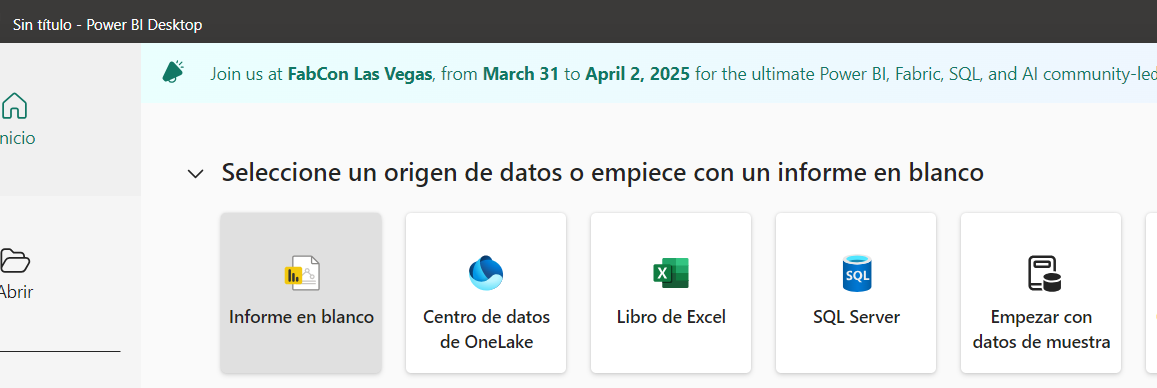
\includegraphics[width=0.8\textwidth]{image/0blanco.png}
		\caption{\textbf{Crear un informe en blanco en PowerBI}}
		\label{fig:1}
	\end{figure}
	
	Después de seleccionar la opción de "informe en blanco", el primer paso es obtener los datos. Aunque existen muchas fuentes de datos, para este proyecto se utilizará los datos de \textit{Analysis Services}, una fuente que se ha trabajado previamente. Para ello, seleccionamos la opción \textit{Analysis Services}, como se muestra en la figura \ref{fig:2}.
	
	\begin{figure}[H]
		\centering
		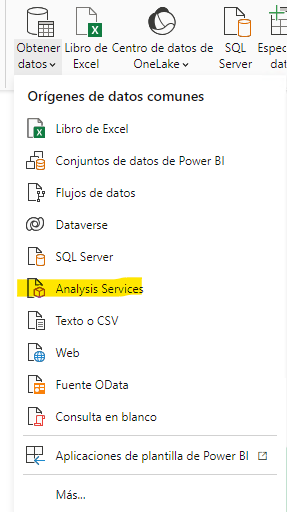
\includegraphics[width=0.4\textwidth]{image/1obetenerdatos.png}
		\caption{\textbf{Selección de Analysis Services}}
		\label{fig:2}
	\end{figure}
	
	\subsection{\textbf{Opciones para Obtener Datos en PowerBI}}
	
	Cuando creamos un informe en \textit{PowerBI}, existen dos opciones principales para obtener los datos: \textbf{Importar} y \textbf{Conectarse en directo}. Cada una de estas opciones tiene ventajas y desventajas según el escenario de trabajo.
	
	\subsubsection{Importar}
	
	La opción \textbf{Importar} permite cargar los datos desde una fuente externa directamente a \textit{PowerBI Desktop}. Los datos se almacenan en el archivo \textit{.pbix}, lo que significa que cualquier transformación o consulta que realicemos se aplicará sobre un conjunto de datos estático, es decir, no se actualizará automáticamente a menos que realicemos una actualización manual. Esta opción es recomendada cuando:
	
	\begin{itemize}
		\item Se trabaja con conjuntos de datos pequeños o medianos que no requieren actualizaciones frecuentes.
		\item Se busca optimizar el rendimiento del informe, ya que los datos están cargados localmente.
		\item Se necesita realizar transformaciones y modelado de datos directamente en \textit{PowerBI}.
	\end{itemize}
	
	A pesar de sus ventajas, esta opción puede generar archivos más grandes y no es la más adecuada cuando los datos cambian constantemente o se requieren actualizaciones en tiempo real.
	
	\subsubsection{Conectarse en Directo}
	
	La opción \textbf{Conectarse en directo}, en cambio, establece una conexión en tiempo real con la fuente de datos, sin necesidad de importar los datos dentro del archivo del proyecto. Las consultas se ejecutan directamente sobre la fuente cada vez que interactuamos con los visuales, lo que garantiza que siempre trabajamos con los datos más recientes. Esta opción es ideal cuando:
	
	\begin{itemize}
		\item Se trabaja con grandes volúmenes de datos que cambian frecuentemente.
		\item Se requiere acceder a datos en tiempo real.
		\item La infraestructura permite mantener conexiones activas y estables con la fuente de datos.
	\end{itemize}
	
	Un ejemplo de esta conexión puede observarse en la figura \ref{fig:3}, donde tras conectarse y autenticarse con las credenciales adecuadas, podemos seleccionar el cubo de datos previamente configurado:
	
	\begin{figure}[H]
		\centering
		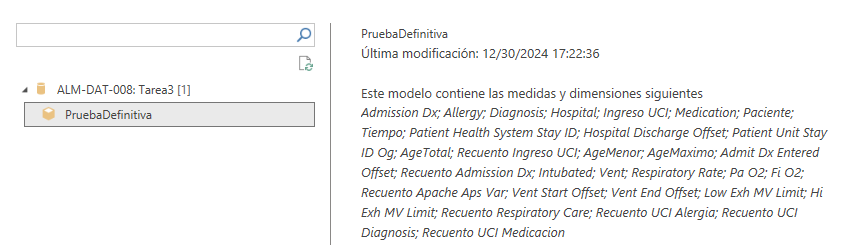
\includegraphics[width=0.75\textwidth]{image/2seleccioncubo.png}
		\caption{\textbf{Selección del Cubo de Analysis Services}}
		\label{fig:3}
	\end{figure}
	
	A pesar de sus ventajas, esta opción puede afectar el rendimiento si la conexión con la fuente no es estable o los volúmenes de datos son muy grandes.
	
	\subsubsection{\textbf{Conclusiones sobre Importar vs Conectarse en Directo}}
	
	Tras analizar las ventajas y desventajas de ambas opciones, se decide experimentar con ambas formas en este proyecto por ser de índole educativo. Al utilizar la conexión directa, encontramos algunas dificultades, al intentar realizar cálculos como el de medias, lo que hizo más compleja la manipulación de los datos. Por otro lado, la opción de \textbf{Importar} ofreció una gran flexibilidad para manejar los datos, y permitió compartir el proyecto de forma más sencilla, especialmente en proyectos donde no se planean actualizaciones constantes en el almacén de datos.
	
	En resumen, para proyectos con datos estáticos o que no requieren actualizaciones frecuentes, la opción de \textbf{Importar} resulta más práctica. Sin embargo, si los datos cambian constantemente o se requieren reportes en tiempo real, \textbf{Conectarse en directo} es la opción más adecuada.
	
	
	\section{\textbf{Pasos Previos a la Creación de Informes}}
	
	Antes de iniciar con la creación de un informe en \textit{PowerBI}, es fundamental tener claros algunos aspectos que facilitarán el desarrollo del proyecto y mejorarán la presentación visual de los datos. Estos pasos previos te ayudarán a optimizar tanto el tiempo de trabajo como la efectividad del informe final.
	
	\subsection{\textbf{Planificación del Contenido}}
	
	Uno de los primeros pasos recomendados es planificar con antelación qué se desea mostrar en cada hoja del informe. Es crucial identificar los indicadores clave o KPIs que se van a visualizar, así como el público objetivo al que va dirigido el informe. Esto te permitirá organizar la información de manera coherente, asegurando que cada página transmita un mensaje claro y conciso. Además, conocer bien los datos con los que vas a trabajar es esencial para seleccionar las visualizaciones más adecuadas. En este proyecto, por ejemplo, se ha trabajado previamente con \textit{Analysis Services}, lo que facilita el conocer las limitaciones de este mismo.
	
	\subsection{\textbf{Personalización del Tema Visual}}
	
	Otro aspecto que facilita el trabajo en \textit{PowerBI} es la personalización del tema visual del informe. Ir a la pestaña \textit{Ver} te permitirá probar diferentes temas predefinidos que \textit{PowerBI} ofrece. Seleccionar un tema que sea coherente con la identidad visual del proyecto o de la empresa puede mejorar considerablemente el aspecto del informe.
	
	Además, \textit{PowerBI} permite la modificación de los temas mediante la opción de \textbf{Modificar temas actuales}. Aquí, puedes cambiar colores, fuentes y estilos para ajustarlos a tus necesidades específicas. Si deseas ir más allá y crear paletas de colores personalizadas, herramientas externas como \href{https://colorhunt.co/}{ColorHunt} y \href{https://paletadecolores.online/mezclar-colores/}{Mezclar Colores} son muy útiles para explorar combinaciones de colores armoniosas y aplicarlas a tu informe (puede ver un ejemplo de personalización en la figura \ref{fig:4}).
	
	\begin{figure}[H]
		\centering
		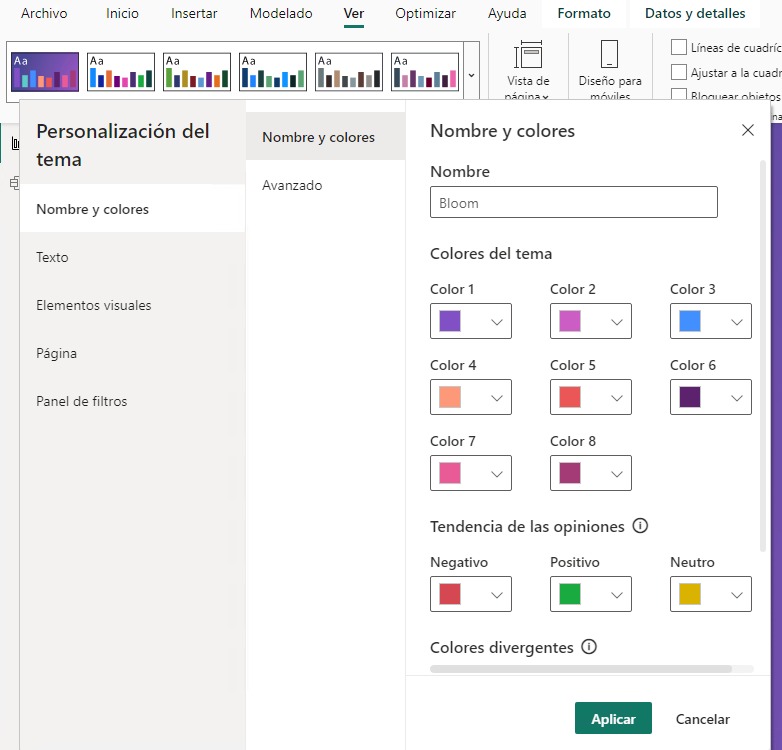
\includegraphics[width=0.93\textwidth]{image/3ver.png}
		\caption{\textbf{Selección de colores y otros temas del proyecto}}
		\label{fig:4}
	\end{figure}
	
	Cabe destacar que posteriormente se puede usar otros colores personalizados pero al definirse previamente se facilita el acceso además de mejora los resultados al pensar en la combinación de color.
	
	\subsection{\textbf{Consejos Adicionales}}
	
	\begin{itemize}
		\item \textbf{Actualizar PowerBI}: El nivel intergráfico a través de los años ha mejorado bastante las opciones personalizadas, comprobar tener la versión más reciente puede ser muy útil.
		\item \textbf{Define una estructura visual}: Intenta mantener una consistencia visual en cada página del informe. Esto incluye utilizar el mismo estilo de gráficos, colores y tamaños para facilitar la lectura y comprensión.
		\item \textbf{Prueba diferentes visualizaciones}: Experimenta con gráficos, tablas y otros tipos de visualizaciones que \textit{PowerBI} ofrece para encontrar la que mejor transmita la información.
		\item \textbf{Optimiza el rendimiento}: Si trabajas con grandes volúmenes de datos, asegúrate de que las visualizaciones y consultas estén optimizadas para evitar tiempos de carga largos.
	\end{itemize}
	
	\section{Creación de un dashboard}
	
	La creación de un \textbf{dashboard} en \textit{PowerBI} depende considerablemente de la fuente de datos y de los elementos que se desean destacar. Si bien no existe un modelo estricto a seguir, es recomendable basar el diseño en los objetivos del informe y en la claridad de la presentación visual. Un buen dashboard debe facilitar la toma de decisiones mediante la visualización efectiva de los datos. 
	
	En \textit{PowerBI}, contamos con una amplia variedad de \textbf{objetos visuales}, cada uno con propósitos específicos, que nos permiten presentar datos de forma clara e interactiva. La versión de PowerBI para enero de 2025 incluye 42 objetos visuales disponibles (ver figura \ref{fig:5}), que permiten construir un informe personalizado.
	
	\begin{figure}[H]
		\centering
		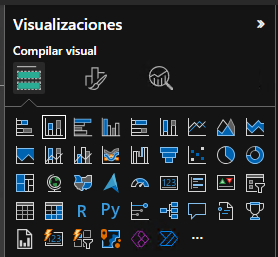
\includegraphics[width=0.5\textwidth]{image/Objetovisual.png}
		\caption{\textbf{Menú con los diversos objetos visuales en PowerBI (2025)}}
		\label{fig:5}
	\end{figure}
	
	A continuación, se presentan algunos de los principales objetos visuales, con una explicación detallada de su utilidad y cómo aplicarlos correctamente en el desarrollo del dashboard.
	
	\subsection{Tarjeta}
	
	La \textbf{tarjeta} es uno de los objetos visuales más utilizados en PowerBI. Es un elemento visual que permite mostrar un solo valor de manera destacada. Suelen utilizarse para resaltar indicadores clave de rendimiento (\textit{Key Performance Indicators}, o KPIs), como ventas totales, ingresos, número de usuarios, o cualquier métrica que se desee monitorear de forma individual.
	
	\textbf{Usos comunes de la tarjeta:}
	\begin{itemize}
		\item Mostrar valores únicos como \textbf{sumas}, \textbf{promedios}, \textbf{máximos} o \textbf{mínimos}.
		\item Resaltar KPIs importantes que requieran atención inmediata.
		\item Comparar resultados históricos o proyectados frente a una meta específica.
		\item Proporcionar una visión rápida de datos numéricos clave que ayuden en la toma de decisiones.
	\end{itemize}
	
	Las tarjetas pueden seleccionarse en el menú anterior en los elementos que cuentan con un rectángulo y dentro unos números 123, se puede ver remarcado en la figura \ref{fig:6} 
	
	\begin{figure}[H]
		\centering
		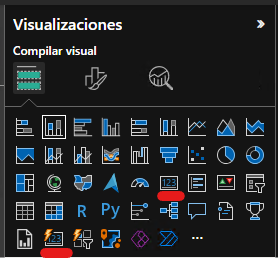
\includegraphics[width=0.5\textwidth]{image/6Tarjeta.png}
		\caption{\textbf{Selección de tarjeta en PowerBI}}
		\label{fig:6}
	\end{figure}
	
	Una vez seleccionado se debe marcar o arrastrar el tipo de dato en "Datos" (revise estar en la pestaña visualizaciones en el apartado de compilar visual/agregar datos a sus objetos visuales), una vez seleccionado se recomienda explorar por cuenta propia el formato de página para cambiar el estilo de la tarjeta (puede ver un ejemplo en la figura \ref{fig:7}).
	
	\begin{figure}[H]
		\centering
		
\includegraphics[width=1\textwidth]{image/7Tarjeta.png}
		\caption{\textbf{Ejemplo de 3 tarjeta en PowerBI}}
		\label{fig:7}
	\end{figure}
	
	Un consejo práctico al usar tarjetas es asegurarse de que los datos mostrados estén claramente definidos y actualizados, ya que suelen ser uno de los primeros elementos que captan la atención de los usuarios.
	
	Además, PowerBI permite combinar tarjetas con otros objetos visuales, como gráficos de barras o líneas, para contextualizar los valores mostrados y proporcionar una mayor profundidad analítica al dashboard. 
	
	\subsection{Gráfico de barras/columnas}
	
	El \textbf{gráfico de barras} es un tipo de gráfico visual que utiliza rectángulos de longitud proporcional a los valores que representan para comparar diferentes categorías. Es especialmente útil para visualizar y comparar datos categóricos y destacar la diferencia entre grupos o categorías de datos. Se usa comúnmente para mostrar comparaciones en métricas como recuentos, promedios o sumas. (ver figura \ref{fig:8}).
	\begin{figure}[H]
		\centering
		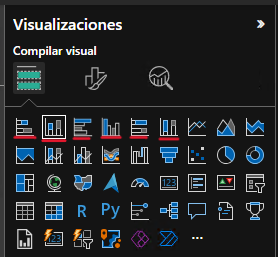
\includegraphics[width=0.4\textwidth]{image/8Tarjeta.png}
		\caption{\textbf{Selección de gráfico de barras o columnas en PowerBI}}
		\label{fig:8}
	\end{figure}
	
	Existen dos principales variantes: el gráfico de \textbf{barras horizontales} y el gráfico de \textbf{columnas} (o barras verticales). En el gráfico de barras horizontales, las categorías están representadas en el eje Y (por ejemplo, géneros como "Male" y "Female"), mientras que en el eje X se colocan las medidas cuantitativas como recuentos, sumas u otras métricas comparables. En el caso de los gráficos de columnas, estos ejes se invierten: las categorías se muestran en el eje X y los valores cuantitativos en el eje Y. (en la figura \ref{fig:9} se puede ver la diferencia en un gráfico de barras y un gráfico de columnas)
	
	\begin{figure}[H]
		\centering
		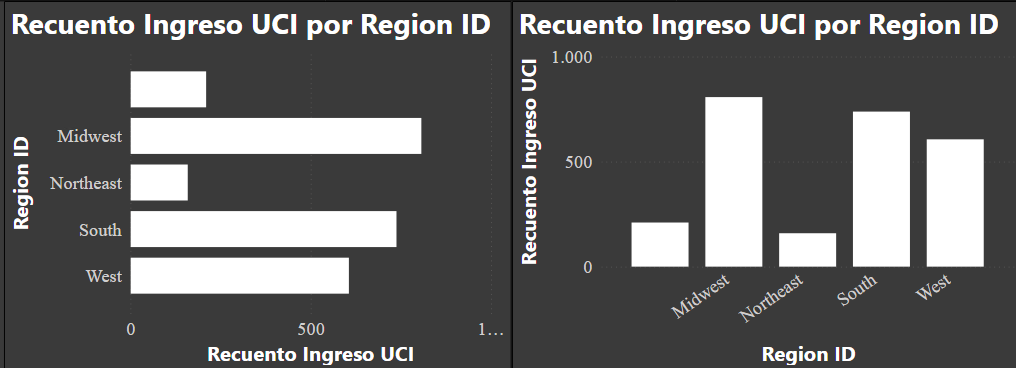
\includegraphics[width=0.8\textwidth]{image/9ejemplo.png}
		\caption{\textbf{Comparación entre barra y columna, para recuento de ingresos según la región del hospital}}
		\label{fig:9}
	\end{figure}
	
	Además, es importante destacar las variaciones de los gráficos de barras, que permiten diferentes formas de representar la información:
	
	\begin{itemize}
		\item \textbf{Gráfico de barras apiladas}: En este tipo de gráfico, los valores de diferentes series se apilan uno encima del otro dentro de cada barra, lo que permite visualizar tanto los totales como las contribuciones de cada serie a ese total. Es útil cuando se desea mostrar la composición de una categoría y cómo los subgrupos contribuyen al todo.
		
		\item \textbf{Gráfico de barras agrupadas}: Muestra múltiples barras una al lado de la otra dentro de una misma categoría, lo que permite comparar directamente varias series de datos dentro de una misma categoría. Este formato es ideal cuando el objetivo es resaltar la comparación entre grupos para cada categoría.
		
		\item \textbf{Gráfico de barras apiladas al 100\%}: Similar al gráfico de barras apiladas, pero en este caso, todas las barras se normalizan para representar el 100\% del total, lo que facilita comparar las proporciones de diferentes series en relación a una categoría, sin importar los valores absolutos.
	\end{itemize}
	
	Cada tipo de gráfico tiene su propio uso recomendado, dependiendo de lo que se desee resaltar. En la figura \ref{fig:10} se muestra un ejemplo utilizando las medidas de \textit{recuento de diagnósticos} y \textit{recuento de medicamentos} para cada tipo de gráfica. A la izquierda, en el gráfico de barras apiladas, se observan ambas medidas apiladas para cada región (incluyendo la región \textit{null}, representada por un espacio en el gráfico). Es fundamental que las medidas utilizadas en este tipo de gráfico tengan sentido al apilarse, como podrían ser datos financieros de distintas fuentes, elementos asignados a un paciente, entre otros. Sin embargo, para el almacén de datos trabajado, esta gráfica no resulta ser la opción más adecuada.
	
	\begin{figure}[H]
		\centering
		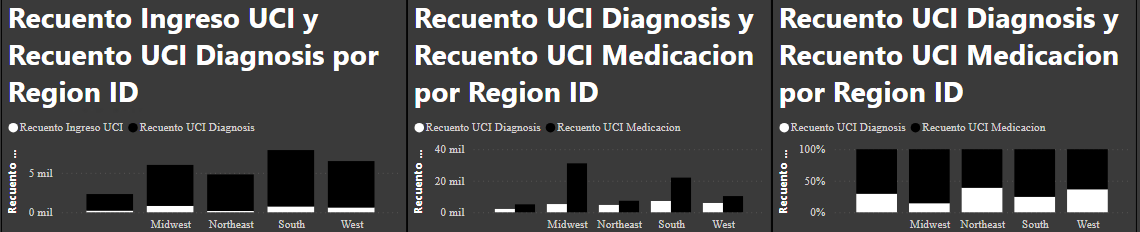
\includegraphics[width=1\textwidth]{image/10casos.png}
		\caption{\textbf{Comparación entre gráficos de barras apiladas, agrupadas y barras 100\% apiladas}}
		\label{fig:10}
	\end{figure}
	
	Por otro lado, el gráfico de barras agrupadas proporciona una mejor visualización al mostrar de manera clara cada medida en su propio nivel dentro de la categoría. Sin embargo, el problema surge cuando una de las medidas, como en el caso de \textit{medicamentos}, presenta valores significativamente mayores, lo que dificulta la apreciación de las demás. Finalmente, la gráfica de barras apiladas al 100\% es una opción interesante cuando se desea comparar proporciones entre las categorías. (la figura \ref{fig:11} muestra como puede quedar el elemento)
	
	\begin{figure}[H]
		\centering
		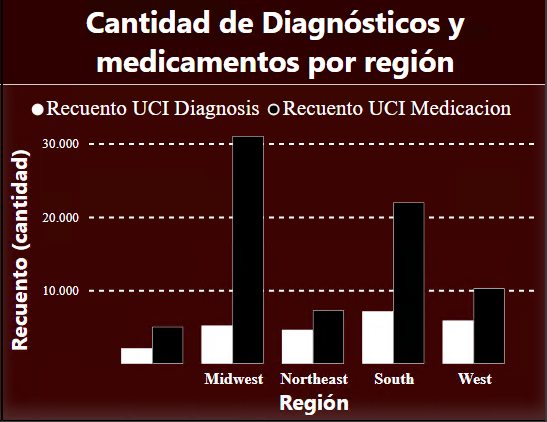
\includegraphics[width=0.6\textwidth]{image/11barras.png}
		\caption{\textbf{Ejemplo de grafico de barras agrupadas con más detalles}}
		\label{fig:11}
	\end{figure}
	
	Es buen momento para destacar la naturaleza interactiva de PowerBI, como se puede ver en la figura \ref{fig:12} al abrir el informe podemos ver muchos datos desde el total de medicamentos usados (75.604), de alergias (2.475) y de ingresos en la UCI (2.520), podemos usar las gráficas para obtener datos más específicos como es el caso de tratar solo con los hospitales de la región Northeast como se ve en la figura \ref{fig:13} al pulsar en el gráfico Northeast todo el informe cambia, adaptándose a los valores del hospital, ahora el total de medicamentos usados son 7.287, se cuenta con 317 alergias entre todos los pacientes y tan solo 159 ingresos.
	
	\begin{figure}[H]
		\centering
		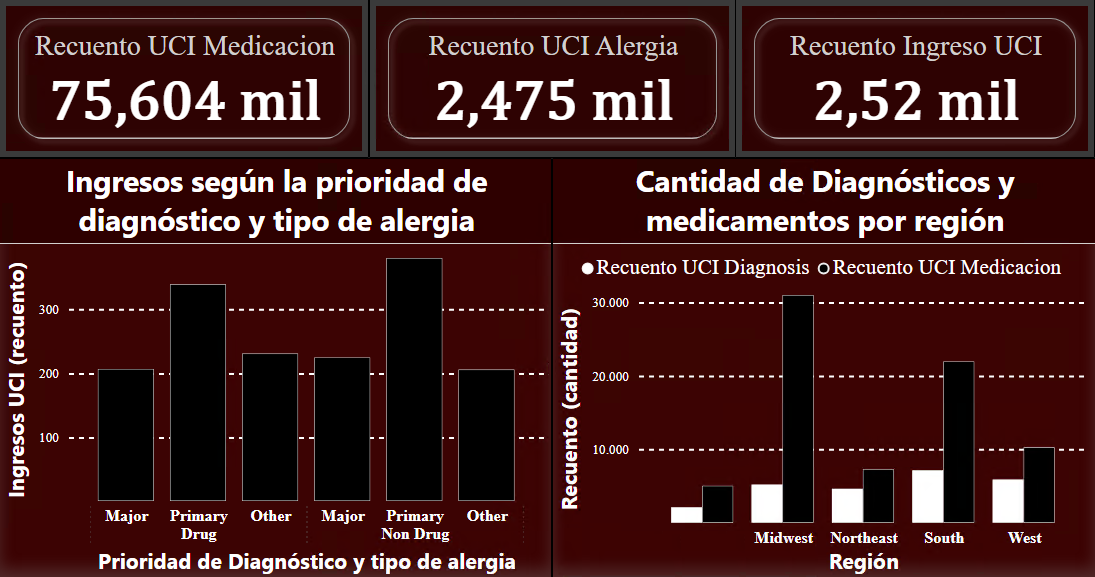
\includegraphics[width=0.6\textwidth]{image/12normal.png}
		\caption{\textbf{Informe sin selección}}
		\label{fig:12}
	\end{figure}
	
	\begin{figure}[H]
		\centering
		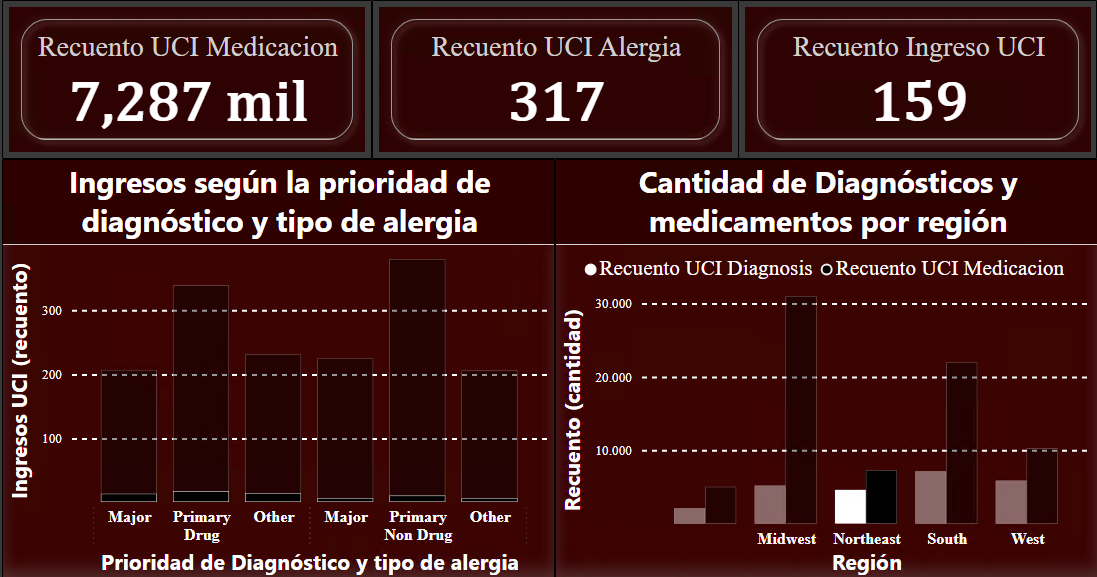
\includegraphics[width=0.6\textwidth]{image/13Northeast.png}
		\caption{\textbf{Informe seleccionando la región Northeast}}
		\label{fig:13}
	\end{figure}
	
	\subsection{Gráfico de líneas/áreas}
	
	Los \textbf{gráficos de líneas} son una representación visual utilizada para mostrar tendencias a lo largo del tiempo u otras dimensiones continuas. Son especialmente útiles cuando se desea resaltar el comportamiento de una métrica en relación a un intervalo, permitiendo identificar cambios, patrones o fluctuaciones en los datos.
	
	En PowerBI, se pueden encontrar varias variaciones de gráficos de líneas y áreas que permiten personalizar la visualización según el propósito del análisis:
	
	\begin{itemize}
		\item \textbf{Gráfico de líneas}: Este tipo de gráfico conecta puntos de datos con líneas, lo que facilita la identificación de tendencias a lo largo del tiempo. Es ideal para visualizar el progreso o la evolución de una métrica, como las ventas o el número de usuarios, en función de una variable continua como el tiempo.
		
		\item \textbf{Gráfico de áreas}: Similar al gráfico de líneas, pero en este caso, el área bajo la línea se rellena con color. Este gráfico es útil cuando se desea enfatizar el volumen total de una métrica, además de su tendencia. El gráfico de áreas permite mostrar tanto el cambio a lo largo del tiempo como la magnitud del total acumulado.
		
		\item \textbf{Gráfico de áreas apiladas}: En este gráfico, se apilan varias áreas una encima de la otra, permitiendo mostrar cómo diferentes categorías contribuyen a un total a lo largo del tiempo. Es útil cuando se desea comparar la evolución de varias series al mismo tiempo, observando tanto los totales como la contribución de cada componente.
		
		\item \textbf{Gráfico de áreas 100\% apiladas}: Similar al gráfico de áreas apiladas, pero en este caso, cada serie se normaliza al 100\%, lo que permite comparar proporciones en lugar de valores absolutos. Es ideal para analizar cómo cambia la composición porcentual de un total a lo largo del tiempo, sin importar las diferencias en magnitud.
		
		\item \textbf{Gráfico de cintas}: Este gráfico es una variación del gráfico de líneas, donde se visualizan las áreas entre líneas para representar la diferencia entre series de datos. Es útil para destacar cambios entre dos o más categorías en función de una variable continua, como el tiempo. 
	\end{itemize}
	
	En este caso la dimensión tiempo es excelente para mostrar este gráfico, no obstante existe un inconveniente con los datos usados y es que contiene la escala de año de datos del 2014 y 2015. La siguiente escala más pequeña es la hora y minuto de entrada al hospital, por lo que termina siendo un caso excesivo de puntos, por lo cual vendrá bien el uso de filtros para este objeto visual, en la figura \ref{fig:14} se puede observar el resultado al filtrar por los ingresos desde las 20:00 hasta las 20:59 cuya cantidad de ingresos sea mayor de 4, este filtro si es usado de modo de práctica pero en una situación real es de interés ver que horas o minutos suele tenerse una mayor cantidad de ingresos.



	\begin{figure}[H]
		\centering
		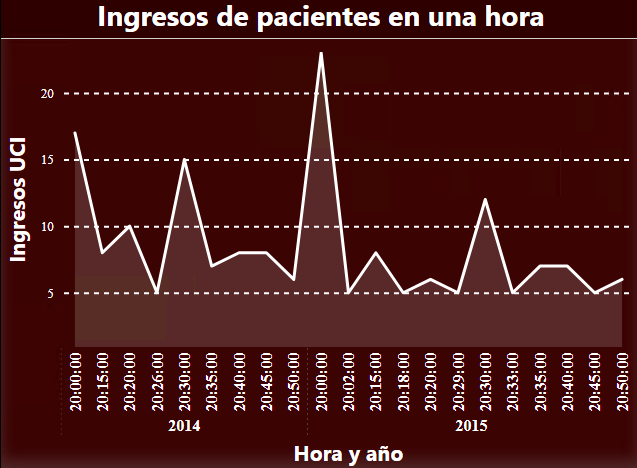
\includegraphics[width=0.7\textwidth]{image/14horas.png}
		\caption{\textbf{Gráfico de área de una hora para los ingresos a las 20:00}}
		\label{fig:14}
	\end{figure}
	
	Los \textbf{filtros} en PowerBI permiten refinar la visualización de los datos, facilitando el análisis de subconjuntos específicos. Existen tres principales tipos de filtros: el filtrado básico, el filtrado avanzado y el filtro \textit{Top N}. El \textit{filtrado básico} permite seleccionar manualmente uno o más valores de una dimensión, restringiendo la visualización únicamente a esos valores seleccionados. Por ejemplo, en un gráfico de áreas que muestra ingresos hospitalarios, se podría filtrar para visualizar únicamente los datos correspondientes a un año específico o a una hora concreta.
	
	El \textit{filtrado avanzado} ofrece una mayor flexibilidad, permitiendo aplicar condiciones más complejas, como filtrar por intervalos de fechas u horas, o establecer criterios numéricos y textuales. Por ejemplo, se podría filtrar los ingresos hospitalarios para mostrar solo aquellos cuya cantidad sea mayor que un valor específico, como en el ejemplo mostrado en la figura \ref{fig:14}. Además, el filtro \textit{Top N} permite mostrar solo los primeros o últimos N valores, ideal para destacar los mayores ingresos hospitalarios en las horas más concurridas o los pacientes con mayor tiempo de estancia. Estos filtros ofrecen un control detallado sobre los datos visualizados, ayudando a los analistas a extraer información precisa y relevante.
	

	\subsection{Gráfico circular/anillo}
	
	El \textbf{gráfico circular}, también conocido como gráfico de torta o pastel, es un objeto visual utilizado para representar proporciones de un total. En PowerBI, se utiliza principalmente para mostrar la contribución de cada categoría a un conjunto completo, distribuyendo las porciones en un círculo donde cada sector representa un porcentaje del total. Este tipo de gráfico es útil cuando se desea comparar rápidamente la magnitud relativa de los diferentes segmentos de datos.
	
	El \textbf{gráfico de anillo} es una variante del gráfico circular. La principal diferencia entre ambos radica en la estética: el gráfico de anillo presenta un espacio vacío en el centro, lo que le da la apariencia de un anillo. En términos de funcionalidad, ambos gráficos se utilizan de manera similar para representar proporciones, pero el gráfico de anillo puede ser más efectivo cuando se quiere agregar información adicional en el centro, como un valor total o una categoría destacada. Este espacio central también puede facilitar la lectura en comparación con el gráfico circular, especialmente cuando hay muchas categorías pequeñas.

	\begin{figure}[H]
		\centering
		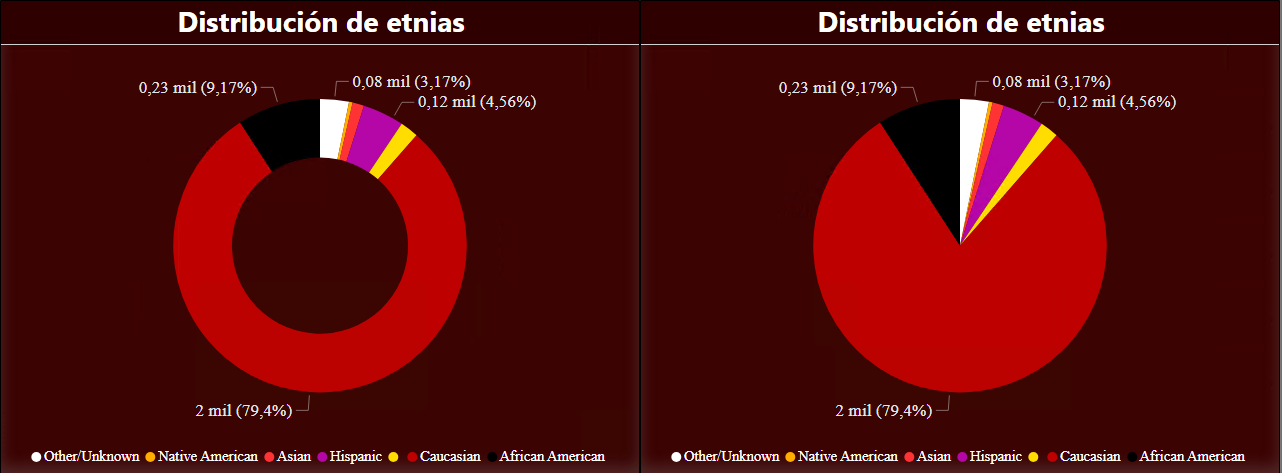
\includegraphics[width=1\textwidth]{image/15circulo.png}
		\caption{\textbf{Gráfico de anillo y círcular para las etnias}}
		\label{fig:15}
	\end{figure}
		
	Como se puede ver en la figura \ref{fig:15} ambos gráficos son muy similares, ambos bastante útiles para representar datos categóricos como es el caso de etnias, mostrando la proporciones relativos de cada categoría, es importante tener en cuenta que cuando hay demasiados segmentos o las diferencias entre ellos son muy pequeñas, los gráficos circulares y de anillo pueden perder claridad. En estos casos, se podría considerar el uso de otro tipo de gráfico que permita visualizar mejor las comparaciones, como un gráfico de barras.
	
	\subsection{Treemap}
	
	El \textbf{Treemap} es un gráfico jerárquico que representa datos categóricos utilizando rectángulos de diferentes tamaños y colores. En PowerBI, se emplea para mostrar la relación entre los diferentes niveles de datos, con el tamaño de cada rectángulo proporcional al valor que representa. Este tipo de visualización es útil cuando se quiere destacar la proporción de cada categoría en comparación con un total, ofreciendo una visión clara de cómo se distribuyen los valores entre las categorías.
	
	Una ventaja del Treemap es que permite mostrar una gran cantidad de datos en un espacio reducido (ver figura \ref{fig:16}), lo que lo convierte en una excelente opción cuando se necesita visualizar múltiples categorías y subcategorías a la vez o rellenar un espacio pequeño en el informe que proporcione valor. Sin embargo, en casos donde las diferencias de tamaño entre los rectángulos sean mínimas, la interpretación puede volverse más compleja, por lo que es importante utilizarlo en contextos donde los datos tengan contrastes claros.
	
	\begin{figure}[H]
		\centering
		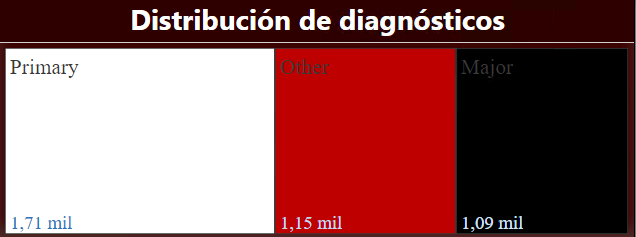
\includegraphics[width=1\textwidth]{image/16treemap.png}
		\caption{\textbf{Ejemplo de Treemap en PowerBI}}
		\label{fig:16}
	\end{figure}

	\subsection{Tabla y Matriz}
	
	En PowerBI, los objetos visuales de \textbf{Tabla} y \textbf{Matriz} son herramientas clave para presentar datos de forma estructurada. Ambos permiten visualizar los datos de manera tabular, pero difieren en su flexibilidad y presentación.
	
	\textbf{La Tabla} es una simple presentación en formato de filas y columnas, donde los datos se muestran sin jerarquías. Es útil cuando se desea ver un listado de valores individuales, permitiendo ordenar, filtrar y explorar los detalles específicos de cada dato. Este formato es ideal cuando el objetivo es mostrar información detallada y específica, como transacciones o registros. (ver figura \ref{fig:17})
	
	\begin{figure}[H]
		\centering
		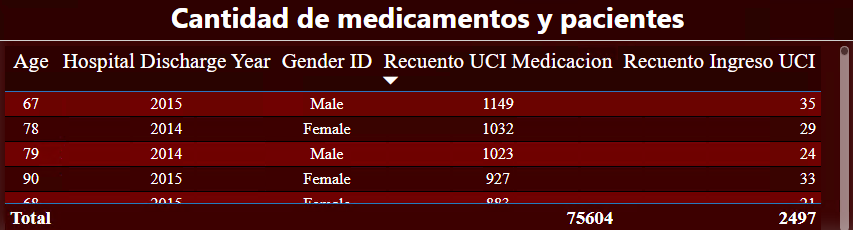
\includegraphics[width=1\textwidth]{image/17tabla.png}
		\caption{\textbf{Ejemplo de una tabla en PowerBI}}
		\label{fig:17}
	\end{figure}
	
	Por otro lado, \textbf{la Matriz} es más avanzada, ya que permite agregar niveles de jerarquía en las filas y columnas. A través de este gráfico, se pueden expandir y contraer grupos de datos, mostrando resúmenes y detalles en un mismo objeto visual. Es especialmente útil para análisis jerárquicos, como la distribución de ventas por región, categoría de producto y subcategoría.
	
	Ambos objetos visuales permiten la personalización de la presentación de los datos, el uso de totales y subtotales, y se pueden complementar con filtros para facilitar el análisis interactivo, en el caso de la figura \ref{fig:17} se decidió filtrar a que el número de medicamentos recetados fuera mayor a 5, para reducir un poco la cantidad de filas, aunque se ópto por no filtrar mucho el contenido de la tabla al poder ser de interés ordenar de menor a mayor el recuento de UCI Medicación para sacar conclusiones.
	
	
	\subsection{Otras herramientas}
	
	Existen varias herramientas en PowerBI que pueden no ser útiles en todos los proyectos si no se cuenta con el contexto adecuado, algunos son:
	
	\textbf{Mapa}: Este objeto visual permite representar datos geográficos de manera visual en un mapa mundial, asignando valores a diferentes ubicaciones geográficas. Es útil cuando se trabaja con datos que incluyen coordenadas o ubicaciones como ciudades o países. Un ejemplo práctico sería el caso de Northwind.
	
	\textbf{Mapa coroplético}: Este tipo de mapa colorea regiones según los valores de los datos, proporcionando una forma visualmente clara de comparar valores entre diferentes áreas geográficas. Por ejemplo, sería útil para visualizar el porcentaje de ventas por estado en un país, donde cada estado se colorea en función de la tasa de ventas.
	
	\textbf{Mapa de Azure}: Similar al mapa básico, pero mejorado con la integración de servicios de Azure Maps. Ofrece una representación más avanzada y detallada de las ubicaciones geográficas, permitiendo realizar análisis espaciales más profundos.
	
	\textbf{Medidor}: Esta herramienta visual representa un único valor en relación con un objetivo, utilizando una visualización de medidor (gauge). Es ideal para hacer un seguimiento del progreso hacia una meta o umbral, como el nivel de cumplimiento de ventas frente a un objetivo.
	
	\textbf{Objeto visual de script de R o Python}: PowerBI permite la creación de gráficos personalizados utilizando scripts en lenguajes como R o Python. Existe ciertos datos que inhabilitan esta opción pero es interesante su existencia
	
	
	\section{Diseño de informes para móviles}
	
	Es interesante destacar que PowerBI ofrece la opción de adaptar los informes para dispositivos móviles de manera sencilla. Desde la pestaña \textit{Ver}, se puede seleccionar la opción \textit{Diseño para móviles}, lo que permite generar automáticamente una versión optimizada del informe para pantallas más pequeñas. Esta funcionalidad es muy útil para asegurar que los datos y visualizaciones se presenten de manera clara y accesible en dispositivos móviles.
	

	
	Aunque la versión para móviles se crea automáticamente, existe posibilidad de modificar y mejorar el diseño como se ve en la figura \ref{fig:18}. Es posible reorganizar los objetos visuales, ajustar su tamaño y disposición para mejorar la experiencia del usuario en pantallas más pequeñas, asegurando que los datos importantes sigan siendo legibles y fáciles de interactuar.
	
	\begin{figure}[H]
	\centering
	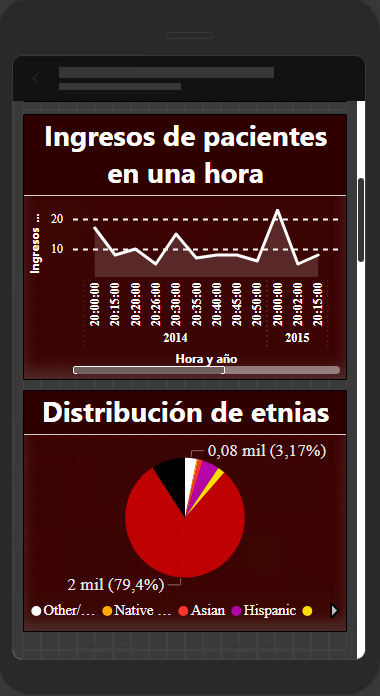
\includegraphics[width=0.6\textwidth]{image/18tabla.png}
	\caption{\textbf{Ejemplo de diseño para moóviles en PowerBI}}
	\label{fig:18}
	\end{figure}
	
	
	\section{Conclusiones}
	
	A lo largo de este documento se ha explorado el uso de PowerBI como una herramienta esencial para la visualización y análisis de datos. PowerBI proporciona una interfaz intuitiva que permite transformar datos complejos en gráficos visuales comprensibles, lo cual es de gran utilidad para la toma de decisiones en entornos empresariales y profesionales. Su capacidad para conectarse con una amplia variedad de fuentes de datos.
	
	Una de las principales fortalezas de PowerBI es la diversidad de gráficos que ofrece, desde barras y líneas, hasta gráficos de área, circulares, de anillo, treemaps, entre otros. Cada uno de estos gráficos tiene su propósito específico y puede adaptarse a distintos tipos de análisis, según lo que se desee resaltar. Además, PowerBI permite la creación de tablas y matrices que facilitan la visualización detallada de datos, lo que lo convierte en una herramienta flexible para presentar información en múltiples formatos.
	
	Otro aspecto relevante de PowerBI son sus capacidades avanzadas de filtrado, que permiten a los usuarios aplicar filtros básicos, avanzados e incluso top N. Esto es particularmente útil cuando se trabaja con grandes volúmenes de datos, ya que posibilita focalizarse en los subconjuntos de información más relevantes. La capacidad de aplicar filtros de manera dinámica mejora la interactividad de los dashboards y la personalización de los análisis.
	
	No obstante, como toda herramienta, PowerBI tiene sus limitaciones. El mayor problema que le encuentro es al obtener datos de una fuente como analysis service limita bastante al deshabilitar bastantes herramientas de modelado, optimización y modificación de datos, sin embargo el uso de datos importados conlleva problemas para almacenés de gran tamaño o relaciones complicadas.
	
	PowerBI es una herramienta poderosa que facilita la creación de visualizaciones interactivas y el análisis de datos de forma fácil. Sus ventajas, como la facilidad de uso, la interactividad, y la capacidad de conectarse a diversas fuentes de datos, lo hacen destacar en el mercado de herramientas de BI. Sin embargo, su rendimiento con datasets extremadamente grandes. A pesar de ello, sigue siendo una opción sólida y ampliamente utilizada en el ámbito profesional.
	
	
	\section{Github y conjunto de instrucciones para su correcto despliegue en SQL Server.}

	Todo el proyecto está accesible en github \cite{depab2024} donde se detalla todos los archivos usados.
	%%%%%%%%%%%%%%%%%%%%%%%%%%%%%%%%%%%%%%%%%%%%%%%%%%%%%%%%%%%%%%%%%%%%%%%%%%%
	\printbibliography
	
	
	%% Back Cover
	
\includepdf[noautoscale=true, width=\paperwidth]{backcover.pdf}
	
\end{document}